\documentclass{Article}
\usepackage[utf8]{inputenc}
\usepackage [danish]{babel}
\usepackage[a4paper, hmargin={2.8cm, 2.8cm}, vmargin={2.5cm, 2.5cm}]{geometry}
\usepackage{eso-pic} % \AddToShipoutPicture
\usepackage{graphicx} % \includegraphics
\linespread{1.2}
\usepackage{amsthm}
\usepackage{amsmath}
\usepackage{url}
\usepackage{tikz}
\usepackage{amsfonts}


\usepackage{listings}


\author{
\Large{dpj482}\\
    \\ \texttt{}
}

\title{
  \vspace{3cm}
  \Huge{CAC assignment 2} \\
  \Large{Christian Møllgaard}\\
}
\usepackage{natbib}
\usepackage{graphicx}

\begin{document}

%% Change `ku-farve` to `nat-farve` to use SCIENCE's old colors or
%% `natbio-farve` to use SCIENCE's new colors and logo.
%\AddToShipoutPicture*{\put(0,0){\includegraphics*[viewport=0 0 700 600]{natbio-farve}}}
\AddToShipoutPicture*{\put(0,602){\includegraphics*[viewport=0 600 700 1600]{natbio-farve}}}

%% Change `ku-en` to `nat-en` to use the `Faculty of Science` header
\AddToShipoutPicture*{\put(0,0){\includegraphics*{nat-en}}}

\clearpage\maketitle
\thispagestyle{empty}

%\newpage



%\lstinputlisting[language=Python, firstline=56, lastline=82]{nbodyphysics.py}

\section{Introduction}
The task of this assignment was to convert the given program to run in parallel on the same generated data. To do this the multiprocessing library is used together with the provided shared memory array shmarray class.

\section{What have changed}
I decided to go with a dynamic model instead of a static model. This choice was due to some hints dropped by other students in class, and I have unfortunately not had the time to test this my self as i went straight for the dynamic model.
%\subsection*{Overall change}
%As a first step i converted V and U to shared memory arrays using the shmarray library, and then made them global. This was needed to make sure the arrays could be called from within the new other processes. The main functions (RD and RD\_visual) then create a process pool. 

%Then i divide U an V into cpu*2 pieces. Then i run the real RD function on each part seperatly and saving the result in another array called Ures and Vres. When all parts have been processes the result arrays are then copied into real array, and then the outer edges gets handled.

\subsection{Data generation}
In the data generation, I converted all returned Numpy arrays to shmarrays, to make them shared memory. To handle an error caused by pickling the shmarrays, I also made U and V global, so I am able to access them from within the other processes. Apart from the changed to U and V I also made result arrays, where i store the result till all processes are done. This way there was no need for a barrier, or the wait for all processes to complete worked as a barrier.

\subsection{The handler}
Before any processing can be done, the data needs to be split up into a few pieces. I split the images based on the amount of desired cpus and a constant, that i have not had the time to optimize, so it is hard coded to 2. At this point i only find the block size, and do not actually split the data yet. I add 1 to the block size to handle when the block size and size of data does not match, and could lead to some rows not getting processed.

The handler then starts the workers with a slight modified version of the original RD function. The part where it updated the values and the edges have been taken out, and it uses the global arrays instead of passed arrays. It gets as argument the block size, and it's index. It then creates views of global arrays, that it uses locally before storing the result in the result array.

The handler wait for all processes to finish this process before moving on, to copying the result back into the original matrices. This is also done in parallel. If I did not have to have global arrays, i could spare alot of time here, by just returning a modified version of the result array as U and V, instead of copying the data back into U and V, but the shmarrays does not really work for me in this way.

After all this is done, I fix the edges.

\section{Result}
I was unable to get all my test data due to bad timing.

To see how the function scales i had planes to find the average with different amount of cpus. There is a clear performance increase, but it does not scale very well with the amount of cpus. Looking at table and figues below, it is easy to see that it does perform faster with more cpus, but it does not scale very well. Some of these bad numbers may be due to the hardcoded cpus*2 workers size.
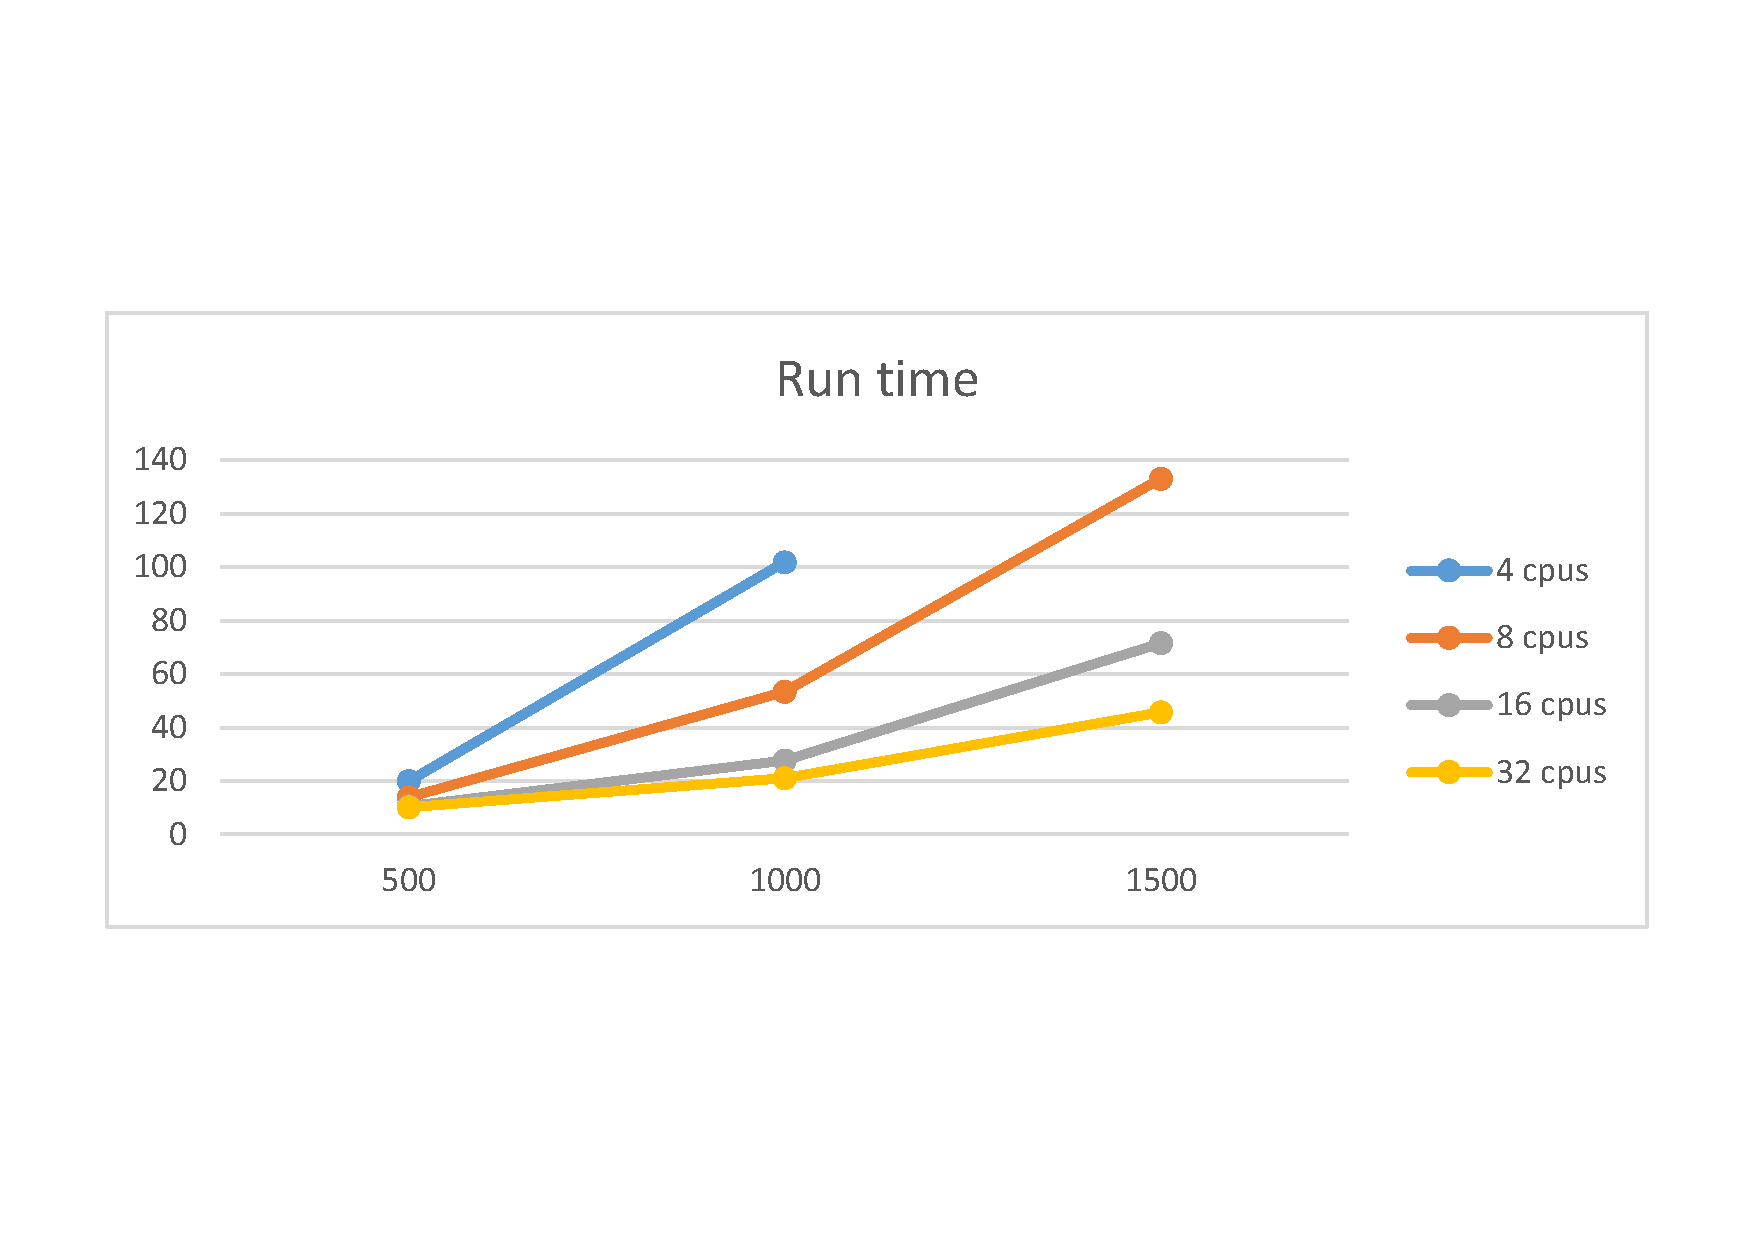
\includegraphics[clip, trim=0 5cm 0 5cm, width=1\textwidth]{plots}\\
\begin{table}[h!]
\centering
\caption{Speedup divided by amount of cpus}
\label{my-label}
\begin{tabular}{|l|l|l|l|l|}
\hline
size & 4 cpus   & 8 cpus   & 16 cpus  & 32 cpus  \\ \hline
500  & 1.071669 & 0.76865  & 0.50444  & 0.262428 \\ \hline
1000 & 0.753961 & 0.720302 & 0.694948 & 0.457387 \\ \hline
1500 & -        & 0.620594 & 0.57769  & 0.452042 \\ \hline
\end{tabular}
\end{table}
\section{conclusion}
The program does run faster with more cpus, but there are some clear scaling issues. Some of these, could be handled, by testing more different constants for the amount of workers. Being able to pickle the shmarrays would speed up the process to somewhat enabling the program to just reassign U and V between the original and a copy.

\end{document}
